\documentclass[11pt,a4paper]{article}
\usepackage{url} % \url command
\usepackage[export]{adjustbox} % Allow specifying image max dimensions
\usepackage{tabularx} % Tables which don't go off the edge of the page
\usepackage[british]{babel} % Quote characters
\usepackage[framemethod=tikz]{mdframed} % Boxes round text
\usepackage[space]{grffile} % Spaces in image filenames

% This turns off hyphenation
\tolerance=1
\emergencystretch=\maxdimen
\hyphenpenalty=10000
\hbadness=10000

% This allows URLs to span multiple lines
\renewcommand{\UrlBreaks}{\do\/\do\a\do\b\do\c\do\d\do\e\do\f\do\g\do\h\do\i\do\j\do\k\do\l\do\m\do\n\do\o\do\p\do\q\do\r\do\s\do\t\do\u\do\v\do\w\do\x\do\y\do\z\do\A\do\B\do\C\do\D\do\E\do\F\do\G\do\H\do\I\do\J\do\K\do\L\do\M\do\N\do\O\do\P\do\Q\do\R\do\S\do\T\do\U\do\V\do\W\do\X\do\Y\do\Z}

\title{MetaboClust User Guide}
\author{Martin Rusilowicz}

\graphicspath{{Images/userguide/}}

\newcommand{\menu}[1]{ \flqq\textit{#1}\frqq}
\newcommand{\icon}[1]{\includegraphics[height=0.75\baselineskip]{#1}}

\newenvironment{detailbox}[1][] {%
	\vspace{\baselineskip}
	\mdfsetup{
		frametitle={%
			\tikz[baseline=(current bounding box.east),outer sep=0pt]%
			\node[anchor=east,rectangle,fill=black!20]%
			{\strut #1};%
			\vspace{\baselineskip}%
		},
		%frametitlebelowskip=2cm,
		%innertopmargin=0pt,
		linecolor=black!50,
		topline=true,
		frametitleaboveskip=0pt,
		rightline=false,
	}
	\begin{mdframed}[]\relax
}
{
	\end{mdframed}
	\vspace{\baselineskip}
}

\begin{document}
\maketitle

\section{System requirements}
For large datasets, a 64-bit system with 8Gb RAM is recommended.

MetaboClust is dependent on the .NET framework. If you are running a recent version of Windows it is more than likely that this is already installed on your computer. If not you will need to download the installer version (see below), or install the framework from one of the following URLs:

\begin{itemize}
	\item \textbf{Windows} -- download the Microsoft .NET from \url{https://www.microsoft.com/net/download}
	\item \textbf{Windows/Linux/Mac} -- download The Mono Project from \url{http://www.mono-project.com/download/}
\end{itemize}

\section{Compiling from source}
MetaboClust is written in C\# using Visual Studio 2015. The source consists of three projects, all of which must be downloaded:

\begin{tabularx}{\linewidth}{l X X X}
	\textbf{Project} & \textbf{Relative path} & \textbf{Contents} & \textbf{Download URL} \\ \hline
	MetaboliteLevels & \url{./MetaboliteLevels/MetaboliteLevels/MetaboliteLevels.csproj} & The main application & \url{https://bitbucket.org/mjr129/metabolitelevels} \\
	MChart & \url{./MChart/MChart/MChart.csproj} & Charting library & \url{https://bitbucket.org/mjr129/mchart} \\
	MGui & \url{./MGui/MGui/MGui.csproj} & Helper library & \url{https://bitbucket.org/mjr129/mgui} \\
\end{tabularx}

From the \textit{downloads} page of each of the projects, select \textit{download repository}. Unzip each of the downloads to a new folder on your disk. If any of the above libraries show as missing make sure they are present in the correct folder, or modify your solution to target the correct path.

MetaboClust also requires the following libraries. Initially these will show as \textit{missing}, but should be downloaded automatically by \textit{NuGet} during the first build. If you have disabled \textit{NuGet} in VS2015 you will need to add the libraries to the solution manually.

\subsection{Running the source}
Build and run the \textit{MetaboliteLevels} project to start the application. Note that due to optimisations being skipped, the application will run considerably slower if the build mode is set to \menu{debug} \textit{and/or} a debugger is attached.

\begin{itemize}
	\item MathNet.Numerics
	\item RDotNet
	\item JetBrains.Annotations
\end{itemize}

\section{Downloading binaries}

If you are not compiling from source, download the application from \url{https://bitbucket.org/mjr129/metabolitelevels/downloads}. The downloads come in two flavours, \textit{Installer} and \textit{Exe}. MetaboClust is a stand-alone application and should not require any special install, hence the \textit{Exe} version is fine. However, if a full installation is preferred, which includes the .NET framework (if required), desktop and start-menu shortcuts and an un-installer, the \textit{Installer} version can be downloaded instead.

\subsection{Running the stand alone version}
After downloading and unzipping, launch \textit{MetaboliteLevels.exe} to start the application.

\subsection{Running the installer}
After downloading and unzipping, run \textit{Setup.exe} and follow the on-screen instructions. The application will be installed using Microsoft ClickOnce -- see \url{https://msdn.microsoft.com/en-us/library/t71a733d.aspx} for troubleshooting and details. After the install you should be able to run the application from your start menu, or by launching \textit{MetaboliteLevels.exe} from the folder you installed the application to.

\begin{detailbox}[Note]
	If an error message appears when you try to start the application, check that the latest version of the .NET framework is installed and working.
\end{detailbox}

\section{Initial setup}
\label{section:ug_initial_setup}
\begin{center}
\includegraphics[max width=0.7\linewidth]{"Images/userguide/initial setup"}
\end{center}

When MetaboClust starts for the first time the initial setup screen shown above is presented. This requires the following information.

\begin{detailbox}[Initial setup options]
	\begin{itemize}
	\item \textbf{Working directory} -- This is where the application stores its data. By default this is the application's home directory. The default value should suffice in most case but can be changed (e.g. if administrator permissions deny read-write access to that folder).
	
	\item \textbf{Path to R} -- MetaboClust uses \textsc{R} to operate and needs to know where R is located. Clicking the \menu{select} button to the right of the text box should automatically detect the location of R and present a drop-down list of the versions of R available. If MetaboClust cannot find an R installation, the path to R will need to be specified manually. Pressing the \menu{select} button (and then, if required, the \menu{browse} option) will prompt you to locate the R installation. On Windows, R is usually located at \texttt{C:\\Program Files\\R\\R-x.x.x\\bin\\x64}, where \texttt{x.x.x} is the version. This folder can be identified by the presence of the R library, \texttt{R.dll}.
	
	\item \textbf{Pathway tools databases} -- MetaboClust uses Pathway Tools databases to make identifications. If any databases are already present on the system MetaboClust can be directed to them here. If no databases are available the \menu{select} button will offer a default location which can be used to put the databases in when you get some.
	\end{itemize}
\end{detailbox}

When you are done, click the \menu{OK} button to commit the selections. MetaboClust detects the presence of errors on most screens. The software will check a connection to R can be established, and check to make sure it has read/write access to the data folders. A greyed out \menu{OK} button indicates an error and a small red arrow should point in the direction of anything amiss. Hover the mouse over the arrow for more details.

\section{Loading data}
\begin{center}
	\includegraphics[max width=0.7\linewidth]{"Images/userguide/loading data"}
\end{center}

Once the initial setup is completed the application will start on the data-load screen shown above. The 
\includegraphics[height=0.5\baselineskip]{Images/userguide/cog} icon in the bottom right of the window presents a drop down menu and the\menu{edit paths and libraries} option here will return you to the \textit{initial setup} screen.

\section{Creating a new session}
A MetaboClust ``session'' is a database of your data, annotations and analyses. You need to create a session before any analysis is performed. Select \menu{create a new session} on the data-load screen to create a new session. The application will walk you through its creation.

\begin{detailbox}[Important note]
	Clicking the \menu{show help} button (or in newer versions the \icon{show help bar} icon) will show a \textit{\textbf{context sensitive}} help bar at the side of the screen containing up-to-date details of the input fields.  For inputs requesting files the \menu{show file format details} button within the help bar describes the expected layout of input files.
\end{detailbox}

Clicking the \menu{Next} button progresses to the next stage of input. If this greyed out a small red arrow will point to anything amiss. Hovering the mouse over the arrow should describe the problem.

\begin{detailbox}[Loading data]
	\begin{itemize}
		\item \textbf{Template} -- Allows you to start from a previous setup. Normally you will start with the \menu{blank template}.
		\item \textbf{Session name} -- For your reference only
		\item \textbf{Data set}
		\subitem \textbf{Source} -- If you have LC-MS data MetaboClust needs to know how the adducts are formed. If the data is not sourced from LC-MS, or automated annotations are not required, then select \menu{Source = Other}, otherwise select the column mode. The \menu{Source = Mixed mode} option allows you to mix modes, but your\menu{peaks} file must then contain an extra column specifying the mode of each peak (\menu{1} or \menu{-1}).
		\subitem \textbf{Intensity matrix} -- The intensity matrix is a grid containing the recorded intensities, with 1 row per observation and 1 column per variable (peak). Row and column headers must be provided and must specify unique names for all observations and peaks. See the help bar as described above for exact details.
		\subitem \textbf{Observation information} -- The observations matrix describes details about each observation, with one observation on each row and one field of information in each column. Row headers should contain the observation IDs as specified for the \menu{Intensities} matrix and column headers should contain the field names. Most fields are optional, but if you don't specify them then some features won't work (for instance batch correction requires the \menu{batch} and/or \menu{acquisition order} fields). Since the exact file format may change with each release, please see the help bar in the software itself for the list of fields (column headers) available.
		\subitem \textbf{Peak information} -- Like the observations matrix, this provides details about each dependent variable. The software refers to all dependent variable as peaks to avoid ambiguity with other variables, such as algorithm parameters. Please see the help bar for the list of fields available.
		\subitem \textbf{Alternate intensities} -- Sometimes another version of your data may be available, such as one prior to noise removal or scaling. The alternate intensities option allows this to be loaded in for quick reference later. Aside from allowing you to view it, it will have no effect on the actual analysis. This feature is not present from version 1.2 as an unlimited number of intensity matrices can be loaded from the file menu.
		\subitem \textbf{Condition names} -- If your experimental groups have unintuitive names, such as ``1'', ``2'' and ``3'' then this allows you to map these to more a readable title.
		\item \textbf{Conditions}
		\subitem \textbf{Specify conditions} -- Details of the experimental groups can be provided here. The conditions should be given as in your \textit{observation information} file or, if present, your \textit{condition names} file. This information is not mandatory, but if specified the software will be able to generate default statistics and filters (described later) for you. If you don't specify the conditions these can still be added manually later.
		\item \textbf{Statistics}
		\subitem \textbf{Auto-create statistics} -- You can choose to generate $t$-tests for your experimental groups against control, as well as pearson correlations of your intensities for each group against time. These options are not available if you didn't specify the conditions earlier. If you don't do this, you can add the statistics manually later.		
		\subitem \textbf{Perform corrections} -- You can add the UV-scale and centre data correction to your pipeline here. This and other corrections can always be added or modified later.
		\item \textbf{Compound libraries} -- These are the compound and pathway libraries used for annotations and pathway analysis. One or more of these must be selected to enable automated annotations. If you don't have any libraries on your system then the list will be empty; see section \ref{section:ug_initial_setup} on how to specify a library folder.
		\subitem \textbf{Adduct libraries} -- These are the adduct libraries used for automated annotations. There are two built into MetaboClust, \textit{All} and \textit{Refined}. The \textit{All} library contains all adducts listed at \cite{kind2010mass}, whilst the \textit{Refined} library contains a common subset of these.
		\item \textbf{Automated identification} -- This will annotate peaks with potential metabolite identifications. The option will be unavailable if required information is missing. If this is selected the \menu{tolerance} must be specified, as well as the \menu{annotation status} to assign the automated annotations. These statuses are \menu{tentative} (unconfirmed identity), \menu{affirmed} (computationally confirmed) or \menu{confirmed} (experimentally confirmed).
		\subitem \textbf{Peak-peak-matching} -- This annotates peaks with other peaks based on $m/z$ similarity and is primarily used to search for related compounds.
		\subitem \textbf{Manual identifications} -- Manual identifications can be loaded from disk. Again, see the help bar for the exact file format. The \menu{annotation status} specified here will only be used if that information is missing from the file itself.
	\end{itemize}
\end{detailbox}

When all the fields you wish to select are complete click the \menu{OK} button to load the data. This may take a few minutes, especially if automated peak-compound annotations are being performed. Saving the session will avoid this delay in future.

\section{Data exploration}
\begin{center}
	\includegraphics[max width=0.7\linewidth]{"Images/userguide/main screen"}
\end{center}

Once you have created or loaded a session you will be presented with the main screen, shown above. As there is no fixed set of steps in analysing a dataset but a brief overview will be presented here. The images here are taken from the analysis of the \textit{Medicago} leaf data. This dataset comprises 184 observations and 2920 peaks, with four experimental groups (C, D, F, B), as well as QC samples. Peaks were automatically annotated using the MedicCyc database \cite{urbanczyk2007mediccyc}.

\section{Univariate statistics}
\label{section:ug_univariate}
Double clicking a peak in the list to the top-left of the window will present a plot of the chosen peak should be displayed to the right. This is a useful first step to ensure the data has loaded correctly.

\begin{detailbox}[Graph controls]
	\begin{itemize}
		\item \textbf{Left or right click} -- Select point or series. Details on that point will be displayed above the graph. Repeatedly clicking will cycle through any overdrawn points.
		\item \textbf{Left click and drag} -- Box-zoom
		\item \textbf{Mouse wheel} -- Zoom in or out
		\item \textbf{Middle click }-- Restore zoom and cancel selection
	\end{itemize}	
	
	The \menu{plot} button above the graph provides plotting options, including exporting the plot to a file and toggling display of the legend.
\end{detailbox}

To show more information about each peak, click the \icon{columns} icon above the peak list. Try showing one of the statistics:

\begin{center}
	\includegraphics[max width=0.5\linewidth]{"Images/userguide/column edit"}
\end{center}

You should then be able to sort the column by that statistic, allowing you to locate the most ``significant'' peaks:

\begin{center}
	\includegraphics[max width=0.5\linewidth]{"Images/userguide/column header"}
\end{center}

Clicking \menu{view as heatmap} will present a heatmap of the column. Note that the peaks are ordered in the heat-map in the same order as the column, so if you sorted the column first, the heat-map will be sorted as well and will appear as a gradient.

\begin{center}
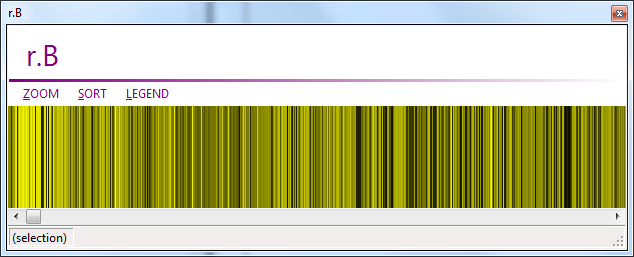
\includegraphics[max width=0.7\linewidth]{Images/userguide/heatmap}
\end{center}

To add univariate statistics, click the \icon{stats} \menu{stats} option from the tool-bar, or select \menu{Database/Workflow/Statistics} from the menu.

\begin{center}
\includegraphics[max width=0.7\linewidth]{"Images/userguide/statistics list"}
\end{center}

Select \menu{New} to create a new statistic.

\begin{center}
	\includegraphics[max width=0.7\linewidth]{"Images/userguide/new statistic"}
\end{center}

\begin{detailbox}[Statistic fields]
	\begin{itemize}
		\item \textbf{Title} -- The title of your statistic. A name will be provided for you if you don't specify one. Clicking the \icon{comment} icon provides space to add detailed comments.
		\item \textbf{Method} -- The statistic to calculate, click the \icon{database} button to the right of the method to define your own methods.
		\item \textbf{Parameters} -- If the method takes any parameters, enter them here. Multiple parameters are separated by commas. Clicking the button next to the text-box displays the parameters as individual inputs rather than a single-line text-box.
		\item \textbf{Target} -- The intensity matrix to work on, from various stages of your analysis. ``origin'' indicates the original intensity matrix you loaded in and will be the only option until you perform data-correction. Items marked with an asterisk designate dynamic sources. Pre-version 1.2 only the latest two intensity matrices are available, which are the latest set of observations (\menu{*final correction}) and trend (\menu{*final trend}).
		\item \textbf{For} or \textbf{Compare} -- Selects the filter to input vector to the statistic, defining the set of observations to use. Click the \icon{database} button to define new filters.
		\item \textbf{Against} -- Only available for bivariate statistics, specifies the second input vector:
		\subitem \textbf{The corresponding time} -- The times corresponding to the first input vector (e.g. to correlate intensity against time)
		\subitem \textbf{A different peak} -- The set of intensities corresponding to the first input vector for a different peak (e.g. to find similar peaks)
		\subitem \textbf{The same peak} -- The set of intensities sourced from different observations on the same peak (e.g. to contrast experimental and control observations).
	\end{itemize}
\end{detailbox}

For instance to calculate the mean of the QC samples select \menu{Method = Mean} and \menu{For = Group is Q}. The \menu{Preview} box allows you to preview the result of your calculation on individual peaks. Select \menu{OK} when you are done.

Click \menu{OK} again to leave the \menu{List editor}. Any new or modified statistics will be recalculated. Edit the columns above the peaks list to show your new statistic.

\section{Exploring annotations}
\begin{center}
	\includegraphics{"Images/userguide/database contents"} 
\end{center}

The set of coloured icons above the list allows paging between the database contents. If automated annotation was chosen when loading the data try selecting the \icon{annot}
 tab and viewing the annotations.
 
 Double click an annotation to view it. Since annotations don't have graphs nothing will be displayed in the top-right, but the secondary list in the bottom-left should update to reflect the selected annotation. Above the secondary list select the \menu{peak} tab to display the peaks associated with the selected annotation. Double-click the peak which appears in the list to plot the peak associated with the annotation.

\begin{detailbox}[Data exploration]
	Almost all of the data in MetaboClust can be explored in this way. The primary list (top) selects items within the dataset, whilst the secondary list (bottom) allows you to explore items within the context of the primary selection. To select an item in the secondary list as the primary selection, click its title above the list:
	\centering
	\includegraphics[max width=0.7\textwidth]{"Images/userguide/promote selection"}
\end{detailbox}	

\section{Multivariate statistics}
An overview of your data can be obtained using PCA. Click the \icon{pca} button in the menu strip to launch the PCA window.

\section{PCA}
The PCA window presents a PCA plot of the dataset. The options to the left control the method of PCA and the display of the scores.

\begin{detailbox}[PCA controls]
	\begin{itemize}
		\item \textbf{Method} -- Switch between PCA and PLSR plots
		\item \textbf{Source} -- Decide whether you are performing PCA on the observations or the variables (the peaks)
		\item \textbf{View} -- Toggle between scores and loadings plots.
		\item \textbf{Legend} -- Select what the colours on the graph represent
		\item \textbf{Corrections} -- View your data with various corrections.\footnote{\label{note:abct}Corrections and trends are defined from the main screen}
		\item \textbf{Input} -- Choose between performing PCA of all observations, or just your trend line (useful for noisy datasets)
		\item \textbf{Observations} -- Select a filter on the set of observations to explore
		\item \textbf{Peaks} -- Select a filter on the set of peaks to explore
		\item \textbf{View on main} -- Displays the selected peak or observation on the main screen.\footnote{\label{note:aspo}Requires an object in the plot to have been selected first}
		\item \textbf{Mark as outlier} -- Applies an observation or peak filter, excluding the selected observation. \footnotemark{b}
		\item \textbf{Next component} -- Views the next principal components
		\item \textbf{Previous component} -- Views the previous principal components
		\item \textbf{Plot options} -- Displays the set of plot options, including toggling display of the legend.
	\end{itemize}
\end{detailbox}

If your data was collected in batches for instance, click the \textsc{Legend} -- the \textsc{Batch} to colour the plot by batch.

Certain subsets of the data can also be selected, click the \textsc{Observations} menu should show a list of observation filters, allowing you to filter on experimental group. As when creating your statistic, if no filters are available you can click \menu{Observations/New filter...} to create a new filter. The same can be done with peak filters by selecting \menu{Peaks/New filter...}.

PCA can also be used for outlier removal. Click an observation in the plot and select the \textsc{mark as outlier} button. A new filter will be created, excluding that observation (or peak) from the dataset.

\section{Data correction}
\label{section:ug_data_correction}
Select \menu{Correct} from the menu-bar of the main screen to open the corrections list. It's empty right now so click \menu{new} to create a new one. 

The data correction window presents a list of data-correction methods, as well as trend generation methods. Data-correction methods, such as scaling and centring act alone, whilst the trend-generators can be used to perform batch correction and control correction.

\begin{detailbox}[Data correction options]
	\begin{itemize}
		\item \textbf{Title} -- As described in section \ref{section:ug_univariate}.
		\item \textbf{Source} -- As described in section \ref{section:ug_univariate}.
		\item \textbf{Method} -- As described in section \ref{section:ug_univariate}.
		\item \textbf{Parameters} -- As described in section \ref{section:ug_univariate}.
		\item \textbf{Source} -- As described in section \ref{section:ug_univariate}.
		\item \textbf{Operator} -- \textit{Only available for trend-based corrections.} The correction takes the form $x\prime = f(x, t)$, where $f$ is defined as $/$ or $-$. Generally a batch correction will use \menu{divide}, and control correction \menu{subtract}.
		\item \textbf{Filter} -- \textit{Only available for trend-based corrections.} Selects the set of points used to generate the trend
	\end{itemize}
\end{detailbox}

The preview window allows you to preview the correction on an individual peak. For trend-based corrections the trend used will be highlighted to the left.

\subsection{Examples}

\subsubsection{QC correction}
Dividing by the mean of the QC samples in the batch is a fairly standard method of correcting for batch-differences in LC-MS, to use this select: \menu{Method = straight line across mean}, \menu{Corrector = Batch}, \menu{Operator = Division} and \menu{Filter = Group is Q}. 

\subsubsection{Background correction}
To perform background correction, as described in chapter \ref{chapter:batchcorrection} select \menu{Method = moving median}, \menu{Corrector = Batch} and \menu{Filter = All}. You will need to enter the window width \menu{w} parameter in this case. Experiment with values to find one that looks good in the plot.

\subsubsection{Scale and centre}
Select \menu{Method = UV scale and centre}. As a direct correction, rather than a trend, there are no other options to choose. This correction should generally be performed \textit{after} batch correction and therefore the \menu{Source} parameter should point to the intensity matrix generated by your batch correction -- QC or Background correction as described above.

\subsection{Viewing corrections}
\begin{center}
	
\includegraphics[max width=0.7\linewidth]{Images/userguide/dataset}
\end{center}

Back on the main screen you will need to select your corrected dataset before your changes can be viewed. Click \icon{dataset button} \menu{dataset} or the drop-down list next to it to select your modified data. You can use the \menu{*Final correction} meta-option to always keep your display up-to-date with the latest correction.

\section{Trend line generation}
You might have noticed the bold lines through 0 on your peak plots (or no lines at all post-version 1.2). These are present because there is currently no trend line defined. Select \icon{trend} \menu{trend} from the tool-bar or \menu{Database/workflow/trends} to define a trend.

You will be presented with a list much like the \menu{correction} window. (Pre-version 1.2 this will containing a \menu{no-trend} entry, click \menu{remove} to get rid of it). Click \menu{new} to create a new trend.

\begin{detailbox}[Trend options]
The \menu{New trend} options are largely the same as those described in section \ref{section:ug_data_correction}.
\end{detailbox}

\subsection{Examples}

\subsubsection{Replicate removal}
The simplest trend is the mean for each time-point. Select \textsc{Method = moving mean} with value \textsc{w = 1}. (\textsc{w} is the window width for the moving mean -- 1 simply indicates a window width of 1, effectively a mean of replicates).

\subsection{Viewing trends}
Back on the main screen you will need to select your trend before your changes can be viewed. Click\menu{trend}
 or the drop-down list next to it to select your modified data. You can use the \menu{*Final trend} meta-option to always keep your display up-to-date with the latest correction.

After selecting your trend any peaks you plot will use the specified trend.
 
\section{Clustering}
Clusters are created in the same way as corrections, statistics or trends. Select the \menu{Cluster} option from the tool-bar of the main window.

\begin{detailbox}
	\begin{itemize}
		\item Title -- As described in section \ref{section:ug_univariate}.
		\item Method -- As described in section \ref{section:ug_univariate}.
		\item Parameters -- As described in section \ref{section:ug_univariate}.
		\item Peaks -- Which peaks to cluster. Since some peaks can interfere with clustering it can be good to filter them out. If you haven't got a suitable filter defined, select the \icon{database} icon next to the list.
		\item Distance -- The distance metric to use. Whilst not used for externally provided algorithms this is still used to calculate certain statistics (next option).
		\item Parameters -- Parameters to the distance metric, as described in section \ref{section:ug_univariate}.
		\item Statistics -- Statistics to calculate for clusters
		\item Source -- As described in section \ref{section:ug_univariate}.
		\item Observations -- The set of observations to use in the clustering vectors
		\item One vector per experimental group -- Normally one vector is created per-peak, select this option to ``split'' the peaks into one vector for each experimental group.
		\item Parameter optimiser -- If the clustering algorithm takes parameters this option can be used to optimise them using statistics such as \textit{silhouette width} or \textit{BIC}.
	\end{itemize}
\end{detailbox}

Alternatively, selecting the \menu{wizard} option from the main menu will guide you through clustering using the \textit{d-k-means++} algorithm, which is a deterministic variant of k-means developed for this software and useful for rapid data exploration.

\subsection{Viewing clusters}
On the main screen click the \menu{cluster} icon above the primary list to view the clusters. Double click a cluster to plot it in the cluster plot area. Note that clusters are always plotted using the vectors with which they were created, so the \menu{trend} and \menu{dataset} visual options will have no effect on the cluster plot.

Clicking a vector within the cluster plot will select the peak associated with that vector as the secondary selection. Alternatively, select the \menu{peaks} tab from the secondary list to show a list of peaks assigned to the selected cluster. Double clicking a peak in this list will plot the peak and highlight it in the cluster plot.

\begin{center}
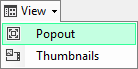
\includegraphics{Images/userguide/popout}
\end{center}

If you want to see a quick overview of all clusters, then click the \menu{View} and \menu{Popout} options above the list of clusters. By default each plot is scaled to fit the plot area, so flat clusters may appear as noisy. To change this and scale all clusters to the same Y-axis, change the plot options by going to the \menu{Prefs} window and setting the \menu{Cluster} -- \menu{Y-axis range} to \menu{Scale to matrix}.

\subsection{Metabolite and pathway exploration}
With a cluster selected, clicking the \menu{compounds} or \menu{pathways} options will show compounds and pathways potentially highlighted by that cluster. Double-clicking these compounds or pathways will highlight the overlap between them and the cluster in the cluster plot. You can show or hide the degree of overlap, or sort clusters by overlap, by selecting the \icon{columns} icon in the secondary list.

A reverse exploration can also be performed, selecting a \menu{pathway} or \menu{compound} in the primary list will plot the trends of the peaks associated with the pathway or compound in the cluster plot. (You can change the \menu{dataset} or \menu{trend} in this case.) As for the clusters, selecting individual trends will plot the actual peak. Selecting \menu{clusters} in the secondary list will show the clusters affected by peaks annotated with the pathway or compound.

\section{General options}

\begin{itemize}
	\item Show or hide observations from experimental groups -- Click the group icon in the main tool-bar to toggle group visibility, or select the \icon{groups} \menu{groups} icon.
	\item Rename groups, peaks, etc. -- Select the \menu{Database} menu to show the database, then edit the group or peak. The groups database can be accessed quickly from the \icon{groups} \menu{groups} icon in the tool-bar. Clicking the name of the session in the top-right of the main screen allows you to rename the session.
	\item Change display options -- Select the \icon{prefs} icon from the tool-bar.
	\item Find out which files were used to create a session -- Select \menu{Help/Session information} from the main menu
	\item Find an individual item -- Click the \menu{name} column of the peaks list and select \menu{filter} from the menu to search for individual items.
	\item Get an overview of the session, including peak and observation counds -- Select \menu{View/Miscellaneous functions} and then \menu{View statistics} from the window that appears.
\end{itemize}

\section{Known bugs}
MetaboClust is beta software. A list of known bugs is maintained on the download page. Please submit any bugs you find to this list.

\end{document}